%----------------------------------------------------------------------
\begin{frame}[c]{Where are we? The big picture}

\begin{itemize}
\item Algorithm Selection
  \begin{itemize}
    \item Portfolios
    \item Algorithm selection (for runtime)
  \end{itemize}
  \item Design decisions:\\ Local Search + Evo. Algorithms + Machine Learning 
  \item Empirical evaluation
  \item AAD for ML
  \begin{itemize}
    \item Hyperparameter optimization and Bayesian optimization 
    \item Neural architecture search (lecture given by Prof. Hutter)
  \end{itemize}
  \item[$\to$] Algorithm configuration 
  \begin{itemize}
    \item[$\to$] Basics 
    \item State of the art 
    \item Best practices 
  \end{itemize}
  \item Combinations of algorithm selection and configurations
  \item Algorithm control 
  \item Algorithm analysis 
  \item Project announcement and questions for exam 
\end{itemize}

\end{frame}
%-----------------------------------------------------------------------


%----------------------------------------------------------------------
\begin{frame}[c]{Preview: Learning Goals}

After this lecture, you should be able to \ldots

\begin{itemize}
  \item \alert{formally} define the algorithm configuration problem \\and discuss its
  complexity
  \item explain the \alert{overtuning} phenomenon and how to avoid it
\pause
\medskip
  \item motivate \& describe the algorithm configuration framework \alert{\paramils{}}
  \item motivate \alert{FocusedILS} and prove its \alert{convergence} property
  \item describe the concept of \alert{adaptive capping}  
\pause
\medskip
  \item describe \alert{application examples} for algorithm configuration
%  \item sketch the ideas of the configurators \gga{} and \irace{}
\end{itemize}
\end{frame}
%----------------------------------------------------------------------



%----------------------------------------------------------------------
\begin{frame}[c,fragile]{Motivation: Sucessful Applications of Algorithm Configuration}

Optimizing speed:

\begin{tabular}{l cc}
\hline
Application & Algorithm (\# params) & Speedup \\
\hline
SAT-based software verification & Spear (26) & \alert{$4.5-500 \times$}\\
AI Planning & LGP (62)	& \alert{$3-118 \times$} \\
Mixed integer programming & CPLEX (76) & \alert{$2-52\times$}\\ 
\hline
\end{tabular}

\pause
\bigskip

Optimizing solution quality:
\begin{itemize}
  \item University timetabling, UBCTT (18 choices)\\
  $\to$ new state of the art; \alert{UBC exam scheduling}
\medskip
\pause
  \item Supervised machine learning, up to 768 design choices\\
   Enables \alert{combined algorithm selection and hyperparameter optimization} (Auto-WEKA and Auto-sklearn) 
\end{itemize}

\end{frame}
%-----------------------------------------------------------------------

\section{Algorithm Configuration} 

%----------------------------------------------------------------------
\begin{frame}[c]{Algorithm Configuration Visualized}

\centering
\scalebox{0.5}{
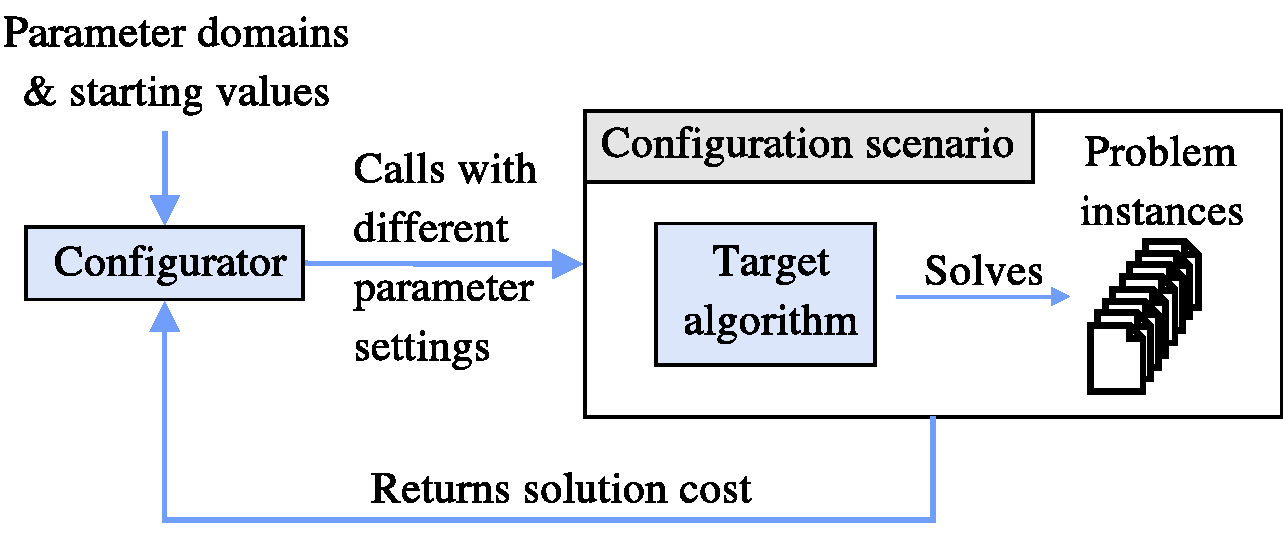
\includegraphics{images/lecture11/Configuration-Process.pdf}
}

\end{frame}
%-----------------------------------------------------------------------


%----------------------------------------------------------------------
\begin{frame}[c]{Algorithm Configuration -- in More Detail}

\bigskip

\centering
\scalebox{0.75}{
\tikzstyle{activity}=[rectangle, draw=black, rounded corners, text centered, text width=8em, fill=white, drop shadow]
\tikzstyle{wideactivity}=[rectangle, draw=black, rounded corners, text centered, text width=10em, fill=white, drop shadow]
\tikzstyle{data}=[rectangle, draw=black, text centered, fill=black!10, text width=8em, drop shadow]
\tikzstyle{myarrow}=[->, thick]
\begin{tikzpicture}[node distance=5cm,thick]
	%PreProcessing
	%\node (Algo) [data] {Algorithm $A$};
	\node (Data) [data] {Instances $\insts$};
	\node (CS) [data, right of=Data, xshift=-0.5cm] {Algorithm $\algo$ and\\ its Configuration\\ Space $\pcs$};
	\node (Select) [activity, below of=Data, node distance=2.0cm] {Select $\conf \in \pcs$\\ and $\inst \in \insts$};
	\node (Run) [wideactivity, right of=Select, xshift=-0.5cm] {Run $\algo(\conf)$ on $\inst$ to measure $c(\conf,\inst)$};
	%\node (Return) [activity, right of=Run, text width=9em] {Return Performance\\ of $A(c)$ on $I'$}; 
	%\node (Data) [data, left of=Select] {Instances $I$};	
	\node (Result) [activity, right of=Run, node distance=4.6cm] {Returns Best\\ Configuration $\hat{\conf}$}; 
	
	\draw[myarrow] (Data) -- ($(Select)+(-0.0,+0.8)$);
	\draw[myarrow] (CS) -- ($(Run)+(-0.0,+0.8)$);
	%\draw[myarrow] (Data) -- ($(Select)+(-2.1,+0.0)$);
	
	%\draw[thick, dashed] (Algo) -- (CS);
	\draw[myarrow] ($(Run.east)+(0.25,0)$) -- (Result);
	\draw[myarrow] (Select) -- (Run);
	%\draw[myarrow] (Run) -- (Return);
	\draw[myarrow] (Run.south) |- ++(0.0,-0.8)  node[above, xshift=-2.2cm] {Return Cost} -| (Select.south);
	
	\begin{pgfonlayer}{background}
    
        % Configuration Process
    	\path (Select -| Select.west)+(-0.25,0.85) node (resUL) {};
    	\path (Run.east |- Run.south)+(0.25,-1.3) node(resBR) {};
    	\path [rounded corners, draw=black!60, dashed] (resUL) rectangle (resBR);
		\path (Run.east |- Run.south)+(-1.5,-1.1) node [text=black!60] {Configuration Task};
    	
    \end{pgfonlayer}
	
\end{tikzpicture}

}

\bigskip

\begin{block}{Definition}
Given a parameterized algorithm $\algo$ with possible parameter settings $\confs$, \pause 
a set of training problem instances $\insts$, \pause 
and a cost metric $m: \confs \times \insts \rightarrow \perf$, \pause 
the algorithm configuration problem is 
to \alert{find a parameter configuration $\conf^* \in \confs$ 
that minimizes $m$ across the instances in $\insts$}.
\end{block}

\end{frame}
%-----------------------------------------------------------------------


%----------------------------------------------------------------------
\begin{frame}[c]{Algorithm Configuration -- Full Formal Definition}

\begin{block}{Definition}
An instance of the algorithm configuration problem
is a 5-tuple $(\algo, \pcs, \instD, \cutoff, m)$ where:
\begin{itemize}
  \item $\algo$ is a parameterized algorithm;
  \item $\pcs$ is the parameter configuration space of $\algo$;
  \item $\instD$ is a distribution over problem instances with domain $\insts$;
\pause
  \item $\cutoff < \infty$ is a \alert{cutoff time}, after which each run of $\algo$ will be terminated if still running
\pause
  \item $m: \confs \times \insts \rightarrow \mathds{R}$ is a function that
  measures the observed cost of running $\algo(\conf)$ on an instance $\inst \in
  \insts$ with cutoff time $\cutoff$ 
%  \item $s$ is a statistical population parameter\\ (e.g., expectation, median,  or variance)
\end{itemize}
\pause
The cost of a candidate solution $\conf\in\confs$ is
%\begin{equation}
%\hat{\conf} \in \argmin_{\conf \in \pcs}
\alert{$c(\conf) = \mathds{E}_{\inst \sim \instD} (m(\conf,\inst))$}.\\
The goal is to find \alert{$\conf^* \in \argmin_{\conf \in \pcs} c(\conf)$}.
%\end{equation}

\end{block}

\end{frame}
%-----------------------------------------------------------------------


%----------------------------------------------------------------------
\begin{frame}[c]{HPO vs AC}

\begin{itemize}
  \item Types of target algorithms 
  \begin{itemize}
    \item HPO deals only with ML algorithms
    \item AC deals with arbitrary algorithms
  \end{itemize}
  \pause
  \item Performance/Cost metrics
  \begin{itemize}
    \item HPO minimizes some kind of loss concerning predictions
    \item AC includes more general metrics, e.g., runtime
  \end{itemize}
  \pause
  \item Randomized Algorithms
  \begin{itemize}
    \item HPO typically ignores that ML algorithms are randomized
    \item Randomized target algorithms in AC will be handled explicitly
  \end{itemize}
  \pause
  \item Prevalence of many categorical \& conditional parameters
  \begin{itemize}
    \item HPO typically considers only continuous parameters
    \item AC addresses much larger configuration spaces
  \end{itemize}
  \pause
  \item Instances and Features
  \begin{itemize}
    \item HPO has no concept of instances
    \item In AC, we optimize $\conf$ across instances
    \item In model-based AC, instance features can be used
  \end{itemize}
\end{itemize}

\pause
\alert{$\leadsto$ HPO $\subset$ AC}

\end{frame}
%-----------------------------------------------------------------------

%----------------------------------------------------------------------
\begin{frame}[c]{Cutoff Time $\kappa$}


Why is it important to impose a cutoff time?
\hands

\pause

\begin{itemize}
  \item Some configurations may be very poor; e.g., never solve an instance
  \pause
  %worst-case runtime to solve an NP-hard problem
  \item Without it, algorithm configuration even becomes undecidable:
\end{itemize}

\begin{block}{Theorem}
  Algorithm configuration with $\kappa = \infty$ is undecidable.
\end{block}

\pause


\begin{block}{Proof by reduction of halting problem to algorithm configuration}
  \begin{itemize}
	\item Define cost of my\_algo with one Boolean parameter:
\vspace*{-0.4cm}
\begin{eqnarray}
\nonumber{}  m(\conf= \langle true \rangle,\inst )&=&
  \begin{cases}
    1, & \text{if $A$ halts on $\pi$}\\
    0, & \text{otherwise}.
  \end{cases}\\
\nonumber{}  m(\conf=\langle false \rangle, \pi) &=& 0.5.
\end{eqnarray}
\pause
\vspace*{-0.6cm}
	\item Then, solving AC for my\_algo and $\inst$ solves the halting problem for $A$:
	\begin{itemize}
	  \item $\conf^* = \langle false \rangle$ implies that $A$ halts on $\pi$ 
	  \item $\conf^* = \langle true \rangle$ implies that $A$ does not halt on $\pi$ 
	\end{itemize}
  \end{itemize}
\end{block}

\end{frame}
%-----------------------------------------------------------------------



%----------------------------------------------------------------------
\begin{frame}[c]{Distribution of Instances}

We usually have a finite number of instances from a given application
\begin{itemize}
  \item We want to do well on that type of instances
  \item Future instances of this type should be solved well 
\end{itemize}

\pause
\bigskip

Like in machine learning
\begin{itemize}
  \item We split the instances into a \alert{training set} and a \alert{test set}
  \item We configure algorithms on the training instances
  \item We only use the test instances afterwards
  \begin{itemize}
    \item[$\to$] unbiased estimate of generalization performance for unseen instances
  \end{itemize}  
\end{itemize}


\end{frame}
%-----------------------------------------------------------------------
%-----------------------------------------------------------------------
\begin{frame}[c]{Recap: Algorithm Parameters}

Parameter Types:
\begin{itemize}
  \item Continuous, integer, ordinal
  \item \alert{Categorical}: finite domain, unordered, e.g., $\{$apple, tomato, pepper$\}$
\end{itemize}

\medskip
\pause

Parameter space has structure
\begin{itemize}
  \item E.g., parameter $\conf_2$ of heuristic $H$ is only active if A is used ($\conf_1 = A$)
  \item In this case, we say $\conf_2$ is a \alert{conditional parameter} with parent $\conf_1$
  \smallskip
  \item sometimes, some combinations of parameter settings are forbidden\\
  		e.g., the combination of $\conf_3 = 1$ and $\conf_4 = 1$ is forbidden 
\end{itemize}

\medskip
\pause

Parameters give rise to a structured space of configurations
\begin{itemize}
  \item Many configurations (e.g., SAT solver \lingeling{} with $10^{947}$ )
  \item Configurations often yield \alert{qualitatively different behaviour}
  \item[$\to$] Algorithm Configuration (as opposed to ``parameter tuning'')
\end{itemize}

\end{frame}
%-----------------------------------------------------------------------

%-----------------------------------------------------------------------
\begin{frame}[c]{Challenges of Algorithm Configuration}

\begin{itemize}
  \item \alert{Structured high-dimensional parameter space}
	\begin{itemize}
	  \item categorical vs. continuous parameters
	  \item conditionals between parameters
	\end{itemize}
  \pause
  \medskip
  \item \alert{Stochastic optimization}
  \begin{itemize}
    \item Randomized algorithms: optimization across various seeds
    \item Distribution of benchmark instances (often wide range of hardness)
    \item Subsumes so-called \emph{multi-armed bandit problem}
  \end{itemize}
  \pause
  \medskip
  \item Some instance sets are \alert{heterogeneous},\\i.e., no single configuration performs well on all instances\\ 
  $\to$ more after the Christmas break
\end{itemize}

%\bigskip
%\pause
%Algorithm Methods:
%\begin{itemize}
%  \item Iterated Local Search, \alert{ParamILS} \lit{Hutter et al., '07 \& '09}
%  \item Genetic algorithm, GGA \lit{Ansotegui et al, '09}
%  \item Iterated F-Race \lit{Birattari et al., '10 - '14}
%  \item Model-based Algorithm Configuration, \alert{SMAC} \lit{Hutter et al., '10 - '14} ($\to$ next week)
%\end{itemize}

\end{frame}
%-----------------------------------------------------------------------





% \hide{
% %-----------------------------------------------------------------------
% \begin{frame}[c,fragile]{Algorithm Configuration}
% 
% Goal: $\hat{\conf} \in \argmin_{\conf \in \confs} \sum_{\inst in \insts} m(\inst, \conf)$
% 
% \bigskip
% 
% \begin{algorithm}[H]
% \Input{%
% instance set $\insts$,
% Algorithm $\algo$ with configuration space $\confs$,
% Initial configuration $\conf_0$,
% performance metric $m$,
% Configuration budget $b$
% }
% \Output{best incumbent configuration $\hat{\conf}$}
% \BlankLine
% \While{$b$ remains} {
% 	$\conf \leftarrow$ select configuration from $\confs$ based on run history $(\conf, \inst, m(\conf,\inst))_i$;\\
% 	$(\conf, \inst, m(\conf,\inst))_k \leftarrow$ run experiments with $\conf$
% }
% 
% \Return{$\hat{\conf}$}
% \caption{Algorithm Configuration}
% \end{algorithm}
% 
% \end{frame}
% %-----------------------------------------------------------------------
% }
% 
% 
% \hide{
% %-----------------------------------------------------------------------
% \begin{frame}[c,fragile]{Simple Random Algorithm Configuration}
% 
% \begin{algorithm}[H]
% \NoCaptionOfAlgo
% \LinesNotNumbered
% \Input{%
% instance set $\insts$,
% algorithm $\algo$ with configuration space $\confs$,
% cost metric $m$,
% Configuration budget $b$
% }
% \Output{best incumbent configuration $\hat{\conf}$}
% \BlankLine
% \onslide<5->
% 	\While{$b$ remains} {
%     \onslide<2->
% 	$\conf \leftarrow$ \alert{sample configuration} from $\confs$ uniformly at random;\\
%     \onslide<3->
% 	\ForAll{\alert{$\inst \in \insts$}}{
% 		Run $\algo(\conf)$ on $\inst$ and measure m(\conf,\inst)$\; 
% 	}
%     \onslide<4->
% 	$cost(\conf) \leftarrow 1/|\insts|$ \sum_{\inst\in\insts} m(\conf,\inst)$ 
%     \onslide<5->
% }
% \onslide<6->
% \Return{configuration $\conf^*$ with minimal $cost(\conf^*)$ of the ones we tried}
% \caption{\textbf{Algorithm 1: Simple Random Algorithm Configuration}}
% \end{algorithm}
% 
% \medskip
% \pause
% 
% \onslide<7->
% Issues:
% \begin{itemize}
%   \item random sampling is not very targetted
%   \item evaluation of $\conf$ on all $\inst \in \insts$ takes a long time 
% \end{itemize}
% 
% \end{frame}
% %-----------------------------------------------------------------------
% 
% 
% 
% 
% %-----------------------------------------------------------------------
% \begin{frame}[c,fragile]{\paramils{} Ideas}
% 
% \begin{itemize}
%   \item \paramils{} = parameter iterative local search
%   \smallskip
%   \item use iterated local search to select configurations\\ (see Lecture 3 on SLS)
%   \begin{itemize}
%     \item iterative improvement as subsidary local search (exploitive greedy search)
%     \item pertubate solution (exploration)\\
%     	  e.g., $n$-random steps in neighbourhood
%   \end{itemize}
%   \smallskip
%   \item evaluate a new configuration only on a necessary amount of instances
%   \begin{itemize}
% 	  \item iteratively increase the number of instances over time to ensure that the current incumbent is indeed a good configuration
% 	  \item aggressively reject configuration if it performs worse than the current incumbent  
%   \end{itemize} 
% \end{itemize}
% 
% \end{frame}
% %-----------------------------------------------------------------------
% 
% 
% 
% 
% %-----------------------------------------------------------------------
% \begin{frame}[c,fragile]{\paramils{} \litw{Hutter et al. 2007,2009}}
% 
% \begin{algorithm}[H]
% \Input{%
% instance set $\insts$,
% Algorithm $\algo$ with configuration space $\confs$,
% Initial configuration $\conf_0$,
% Configuration budget $b$,
% performance metric $m$
% }
% \Output{best incumbent configuration $\hat{\conf}$}
% \BlankLine
% $\hat{\conf} \leftarrow \conf_0$; \\
% $\conf \leftarrow \conf_0$; \\
% \While{$b$ remains} {
% 	$\conf \leftarrow$ pertubation(\conf)$; \\ %\tcp*{n-random steps in neighbourhood}\\
% 	$\conf \leftarrow$ local\_search(\conf);\\
% 	\If{$\conf$ is better than $\hat{\conf}$}{ 
% 		$\hat{\conf} \leftarrow \conf$;
% 	}
% }
% 
% \Return{$\hat{\conf}$}
% \caption{\paramils}
% \end{algorithm}
% 
% \end{frame}
% %-----------------------------------------------------------------------
% 
% 
% }


\section{ParamILS: iterated local search in parameter space}


%-------------------------------------------------------------
\begin{frame}[c,fragile]{A Simple Manual Approach for Configuration}

%\begin{itemize}
%\item Choose a ``representative'' benchmark set for tuning
%
%\pause
%\medskip
%
%\item Perform iterative manual tuning:
%

\NoCaptionOfAlgo
\LinesNotNumbered
\begin{algorithm}[H]
        Start with some configuration $\conf$\;
        \onslide<4->
  \Repeat{no more improvement possible (or ``good enough'')}{
    \onslide<2->
    Modify a single parameter\;
    \onslide<3->
    \If{results on benchmark set improve}
    {
            keep new configuration\;
    }
        \onslide<4->
  }
\caption{\textbf{Algorithm 1: Manual Greedy Algorithm Configuration}}
\end{algorithm}

\onslide<5->
\medskip
What would you call this approach? \hands\\
\smallskip
\onslide<6->
$\leadsto$ Manually-executed \alert{first-improvement local search}

\medskip

\onslide<7->
How could we improve this approach?\hands\\ 
\smallskip
\onslide<8->
$\leadsto$ Any of the advanced SLS methods from Lecture 4.

\end{frame}
%-------------------------------------------------------------




%-------------------------------------------------------------
\begin{frame}[c,fragile]{The \paramils{} Framework}

\vspace*{-0.3cm}ParamILS = Iterated Local Search in parameter configuration space
\bigskip

\onslide<2->
\NoCaptionOfAlgo
\LinesNotNumbered
\begin{algorithm}[H]
        Choose initial parameter configuration $\conf$\\
        Perform \cemph{teal}{subsidiary local search} on $\theta$\\
        \onslide<6->
  \While{time budget left}{
    \onslide<3->
    $\conf_{lm} \leftarrow \conf$ ~~~~~~~~~~~~~~~~~~~~~~~~~~~~~~~~~~~~// last local optimum\;
    \onslide<4->
    Perform \cemph{orange}{perturbation} on $\theta$\;
    Perform \cemph{teal}{subsidiary local search} on $\theta$\;
    
    Based on \cemph{green!60!black!100}{acceptance criterion},
	    keep $\conf$ or revert to $\conf:=\conf_{lm}$
        \onslide<5->
        
   With probability $p_{restart}$ randomly pick new $\theta$ 
           \onslide<6->
  }
\caption{\textbf{Algorithm 2: ParamILS}}
\end{algorithm}
        \onslide<7->

\bigskip
$\leadsto$ Performs \alert{biased random walk over local optima}

\end{frame}
%-------------------------------------------------------------



%-------------------------------------------------------------
\begin{frame}[c,fragile]{The \paramils{} Framework}

\paramils{} is an algorithm framework made up of building blocks:

\begin{itemize}
  \item In practice, \paramils{} implements these as follows:
  \begin{itemize}
    \item \cemph{teal}{Subsidiary local search}: greedy first improvement
    \item \cemph{orange}{Perturbation}: 3 random moves in 1-exchange neighbourhood
    \item \cemph{green!60!black!100}{Acceptance criterion}: always improve better configuration
    \item Note: these choices are not necessarily optimal \ldots
  \end{itemize}
  
  \pause
  \bigskip
  
  \item \paramils{} performs a sequence of \emph{pairwise} comparisons
  \begin{itemize}
    \item \alert{is $\conf'$ better than current $\conf$}?
    \item 2 instantiations that answer this question based on different runs of $\conf$ and $\conf'$: \alert{BasicILS} and \alert{FocusedILS}
  \end{itemize}   
\end{itemize}


\end{frame}
%-------------------------------------------------------------



%-----------------------------------------------------------------------
\begin{frame}[c,fragile]{BasicILS(N)}
%: one instantiation of ``is $\conf'$ better than $\conf$?''

\begin{itemize}
  \item \alert{BasicILS(N)} uses a pretty basic comparison: \textit{better$_N(\conf', \conf)$}:
  \begin{itemize}
    \item Compare $\conf'$ and $\conf$ based on $N$ instances 
\pause
	\item How does this relate to cross-validation? \hands
  \end{itemize}  

\bigskip
\pause
    \item Problem: How to set $N$? Problems of large $N$? Small $N$? \hands
    \pause
		\begin{itemize}
			\item Problem of large $N$: evaluations are slow
			\item Problem of small $N$: overfitting to a small set of instances
%			\item What is the problem of choosing $N$ too small?
%			\begin{itemize}
%				\item[\voteblue{}] Evaluation of $c_N(\conf)$ is too fast
%				\item[\voteyellow{}] Overfitting to a small set of instances
%			\end{itemize}
			\item[$\leadsto$] Tradeoff: Choose $N$ of moderate size 
		\end{itemize}
%    \item[$\to$] too small $N$ will lead to overfitting on a small set of instances
%    \item[$\to$] too large $N$ will need to much time to evaluate

  \end{itemize}
\end{frame}
%-----------------------------------------------------------------------


%-----------------------------------------------------------------------
\begin{frame}[c,fragile]{BasicILS(N)}


Question: \alert{Which} $N$ instances should we use? \hands
\begin{enumerate}
	\item $N$ different instances for each configuration
	\item The same set of $N$ instances for the entire run
\end{enumerate}

\bigskip
\pause
  Answer: the same $N$ instances, so that we compare apples with apples
  \begin{itemize}
	\item[] (but: using the same instances can also yield overtuning) 
  \end{itemize}
\bigskip
  
  
 If we sampled different instances for each configuration:
  \begin{itemize}
	\item Some configurations would randomly get easier instances
	\item Those configurations would look better than they really are
  \end{itemize}

%  \item What is the problem of sampling \\different instances for each configuration?
%\begin{itemize}
%	\item[\voteblue{}] We don't have that many instances
%	\item[\votepurple{}] It's costly to sample instances for every configuration
%\end{itemize}
%\medskip
%\pause
%$\leadsto$ we need to compare apples with apples

\end{frame}
%-----------------------------------------------------------------------



%-----------------------------------------------------------------------
\begin{frame}[c,fragile]{BasicILS(N)}

Question: For randomized algorithms, how should we set the seeds? \hands
\begin{enumerate}
	\item Sample a new seed for each algorithm run
	\item Fix the seeds together with the instances
\end{enumerate}
\bigskip
\pause
Answer: just like for instances, fix them to compare apples to apples

\bigskip
\pause
In summary, for each run of BasicILS(N): \\pick $N$ (instance, seed) pairs and use them for evaluating each $\conf$.\\
\pause
(Different BasicILS runs can use different instances and seeds.)

\end{frame}
%-----------------------------------------------------------------------


%-----------------------------------------------------------------------
\begin{frame}[fragile]{The concept of overtuning}

Very related to overfitting in machine learning 
\begin{itemize}
	\item Performance improves on the training set
	\item Performance does not improve on the test set, and may even degrade
\end{itemize}	

More pronounced for more heterogeneous benchmark sets 
\begin{itemize}
	\item But it even happens for very homogeneous sets
	\item Indeed, one can even overfit on a single instace, to the \alert{seeds} used for training 
\end{itemize}	

\end{frame}
%-----------------------------------------------------------------------

%-----------------------------------------------------------------------
\begin{frame}[fragile]{Overtuning Visualized}

\begin{itemize}
	\item Example: minimizing SLS solver runlengths for a single SAT instance
	\item \alert{Training cost}, e.g., with N=100:\\average runlengths across 100 runs with different seeds
	\item \alert{Test cost} of $\hat{\conf}$ here based on 1000 new seeds 
\end{itemize}	

\pause


\begin{center}
\only<2>{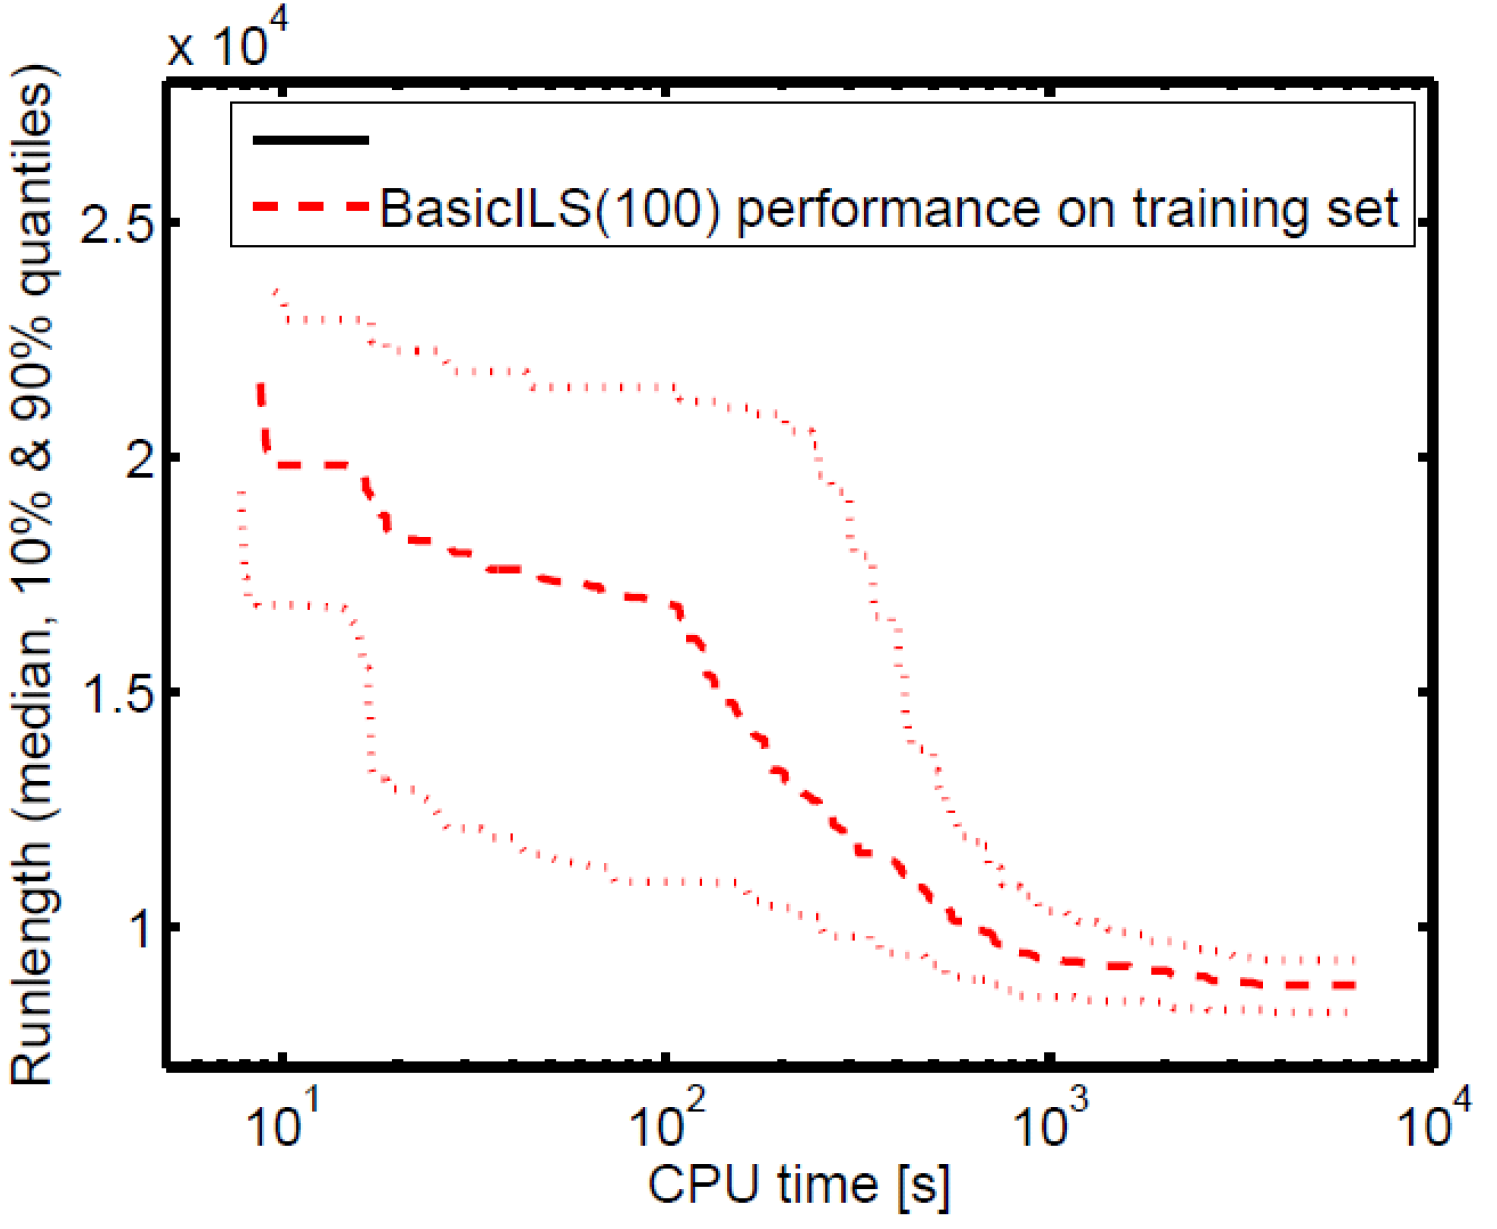
\includegraphics[scale=0.13]{images/lecture11/basicils100_training.png}}
\only<3>{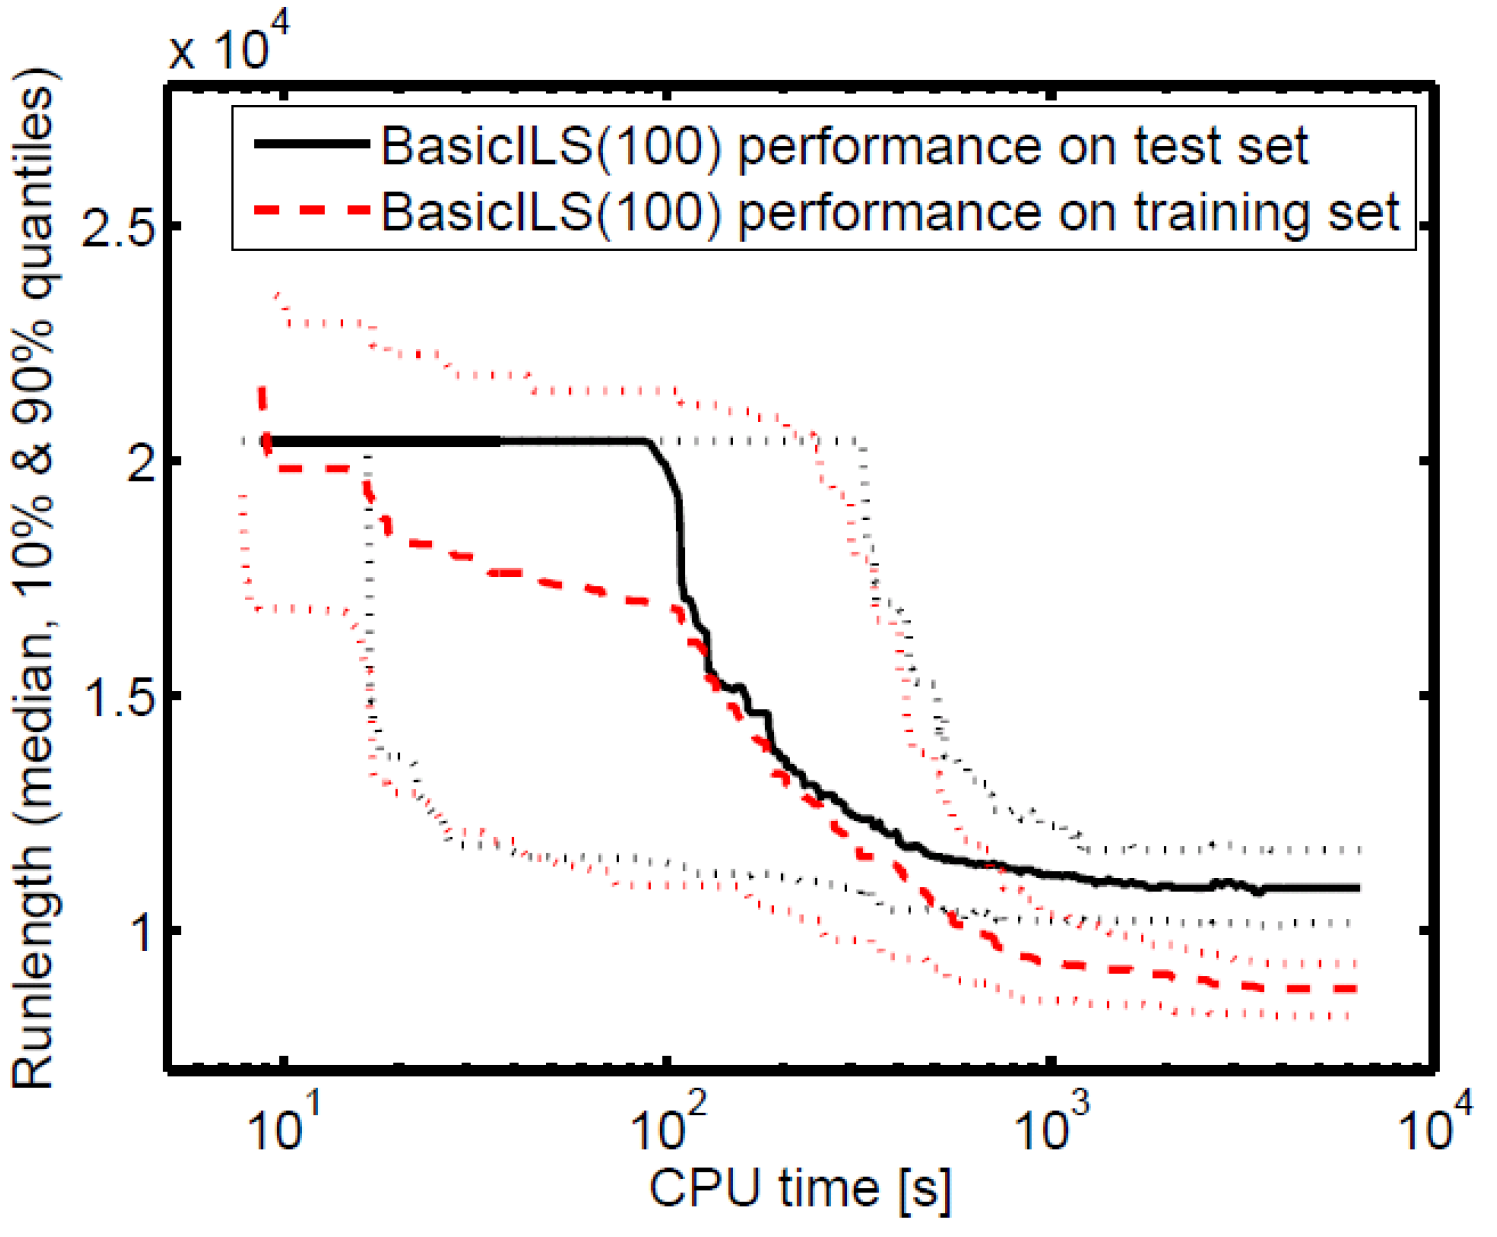
\includegraphics[scale=0.13]{images/lecture11/basicils100_training_and_test.png}}
\end{center}


\end{frame}
%-----------------------------------------------------------------------

%-----------------------------------------------------------------------
\begin{frame}[fragile]{BasicILS(N) Test Results with Various N}

\begin{itemize}
	\item Example: minimizing SLS solver runlengths for a single SAT instance
	\item \alert{Training cost}, e.g., with N=?:\\average runlengths across N runs with different seeds
	\item \alert{Test cost} of $\hat{\conf}$ here based on 1000 new seeds 
\end{itemize}	

\pause

\begin{multicols}{2}
\begin{center}
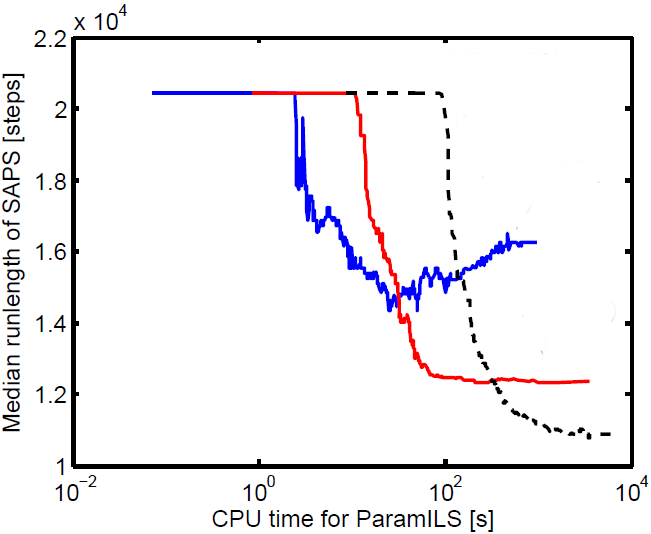
\includegraphics[scale=0.2]{images/basicils_unlabled.png}
\end{center}
\columnbreak{}
\pause
Which of these results corresponds to $N=1$, $N=10$, and $N=100$?\\
\hands

\pause
\medskip

\begin{enumerate}
	\item N=1: blue, N=10: red,\\ N=100 dashed black
	\item N=1: dashed black,\\ N=10: red, N=100 blue
\end{enumerate}

\pause
Correct Answer: 1


\end{multicols}


\end{frame}
%-----------------------------------------------------------------------

%-----------------------------------------------------------------------
\begin{frame}[fragile]{Overtuning is Stronger For Smaller Training Sets}

\begin{center}
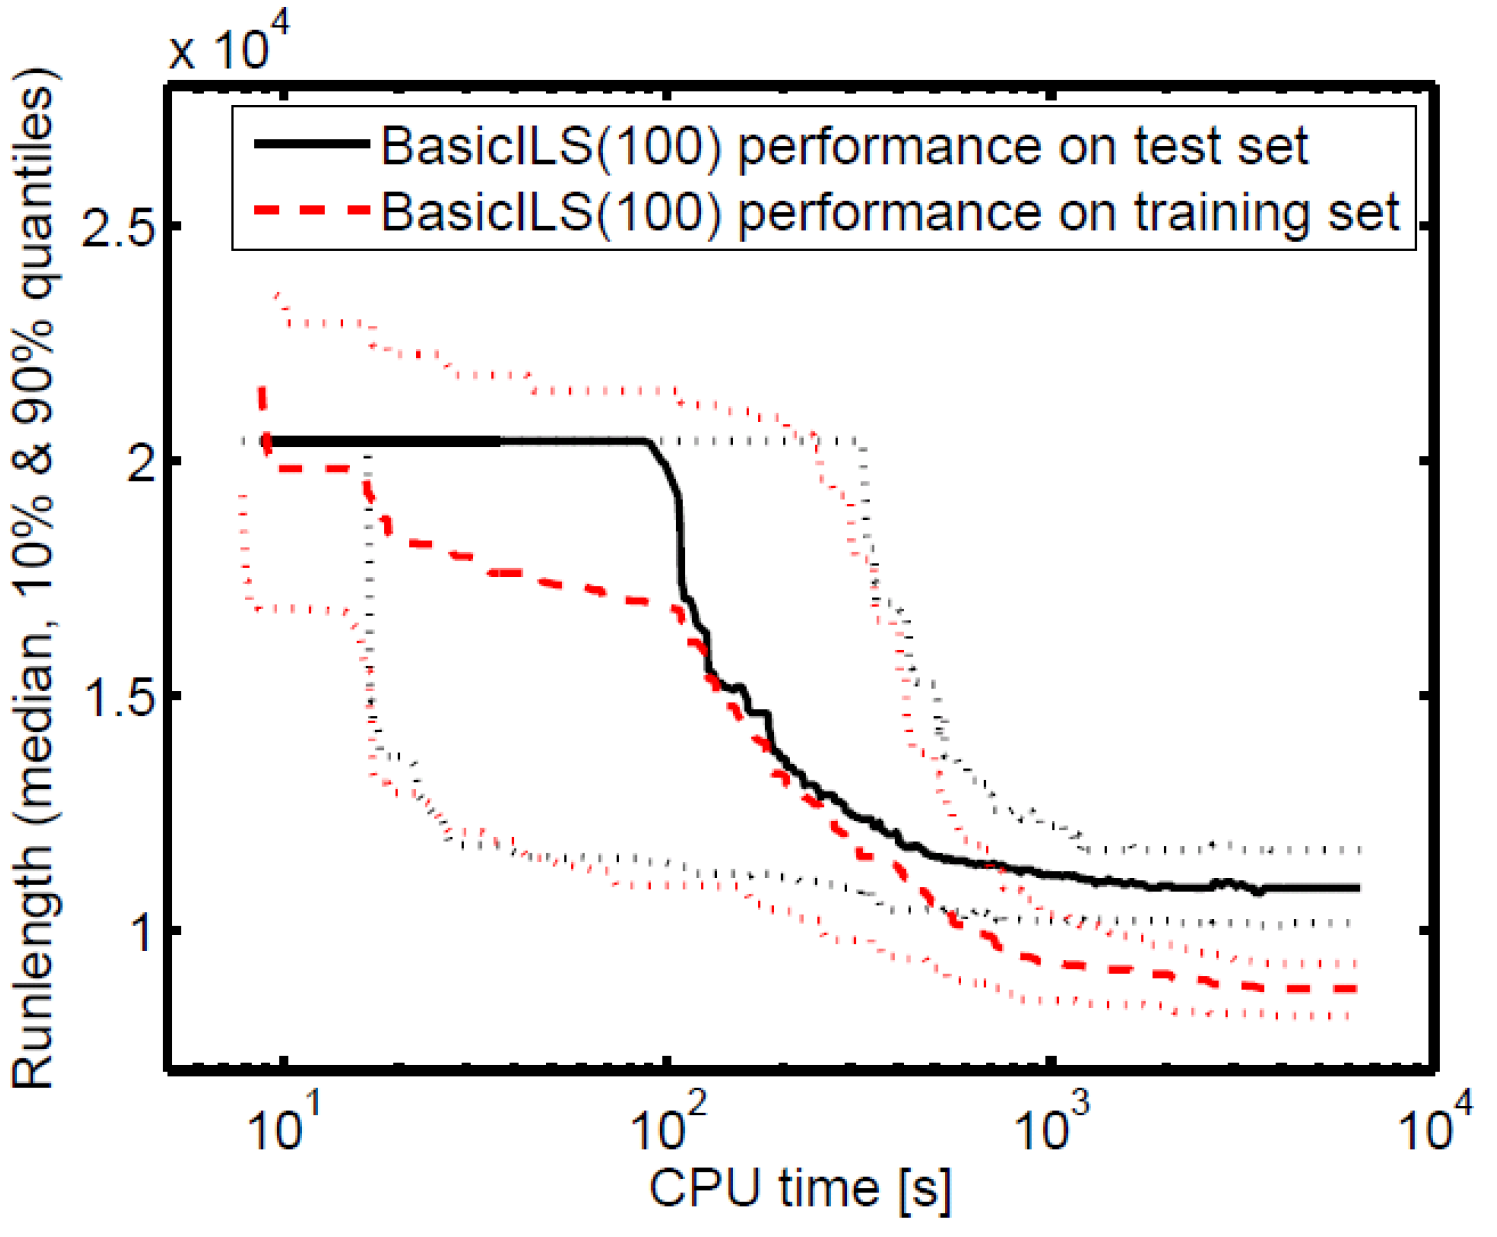
\includegraphics[scale=0.15]{images/lecture11/basicils100_training_and_test.png}
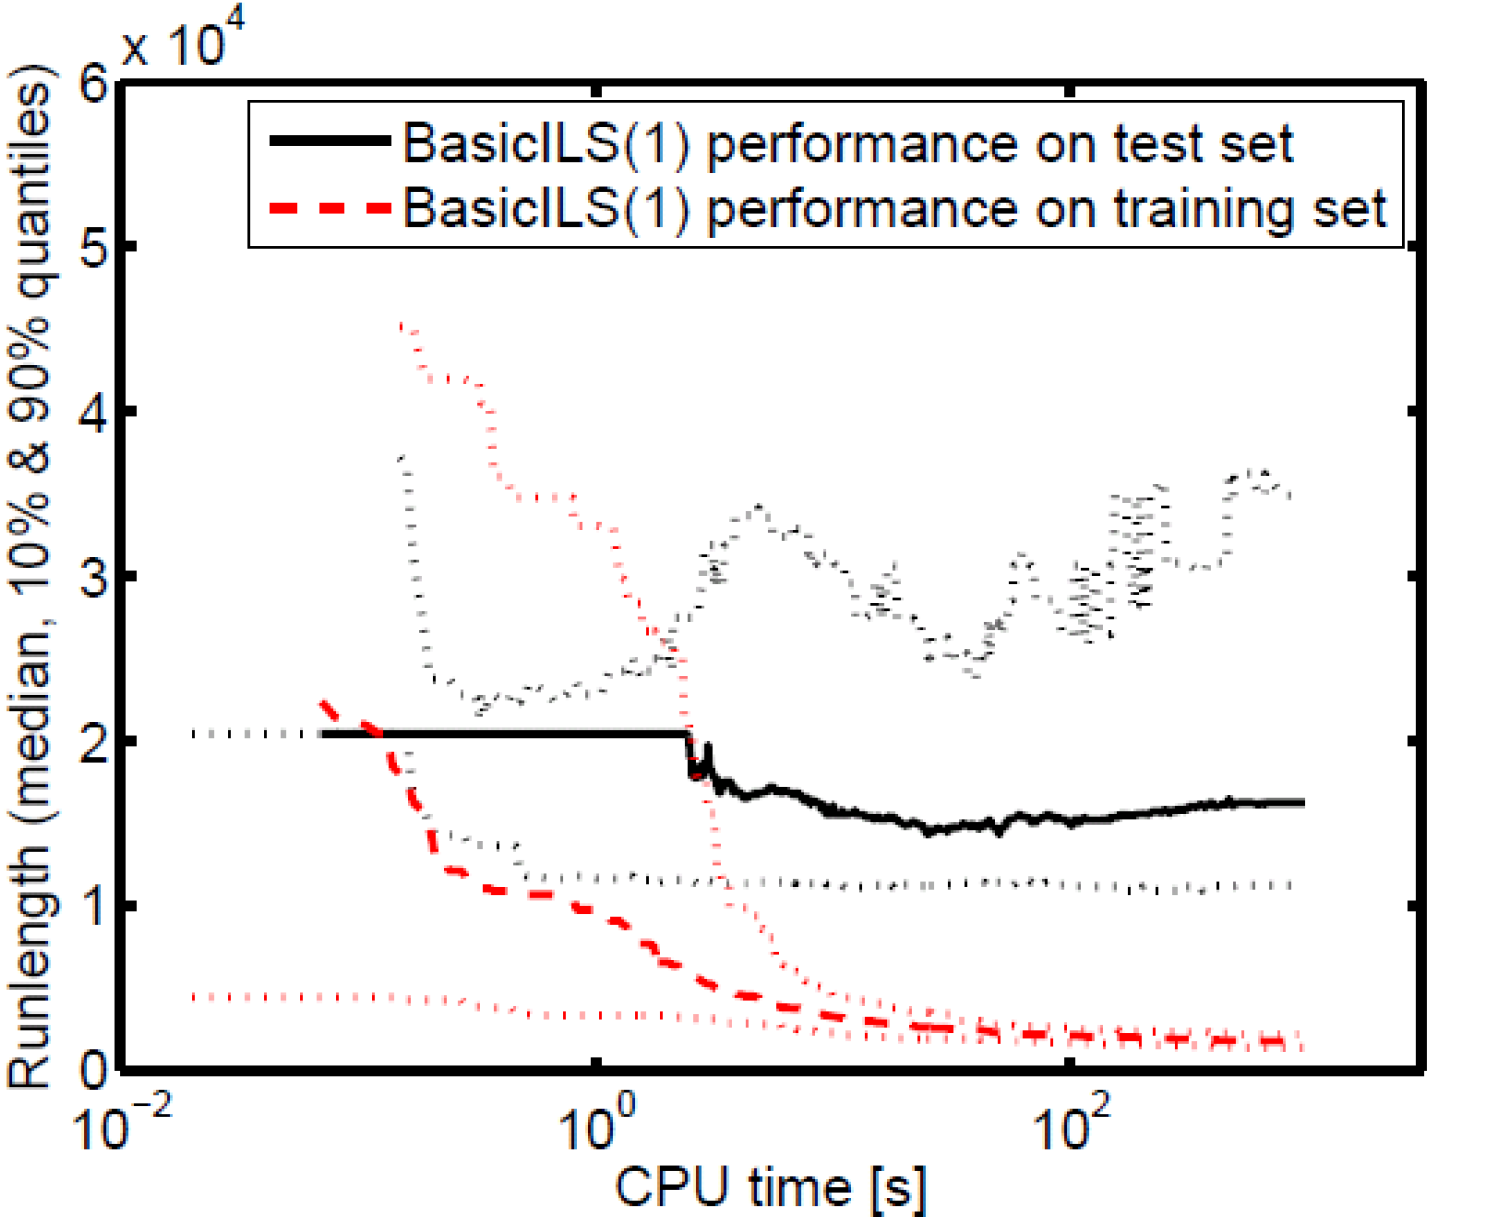
\includegraphics[scale=0.15]{images/lecture11/basicils1_training_and_test.png}
\end{center}

\end{frame}
%-----------------------------------------------------------------------




%-----------------------------------------------------------------------
\begin{frame}[c,fragile]{FocusedILS}

Intuition: get the best of both worlds
\begin{itemize}
	\item Perform more runs for good configurations
	\begin{itemize}
	  \item[-] to avoid overtuning
	\end{itemize}
	\item Quickly reject poor configurations
	\begin{itemize}
	  \item[-] to make progress more quickly
	\end{itemize}
\end{itemize}

\pause

\begin{block}{Definition: $N(\conf)$ and $c_N(\conf)$}
\alert{$N(\conf)$} denotes the number of runs executed for $\conf$ so far.\\
\alert{$\hat{c}_N(\conf)$} denotes the cost estimate of $\conf$ based on $N$ runs.
\end{block}

\pause
In the beginning: $N(\conf)=0$ for every configuration $\conf$

\end{frame}

%-----------------------------------------------------------------------



%-----------------------------------------------------------------------
\begin{frame}[c,fragile]{FocusedILS}


\begin{block}{Definition: domination}
\alert{$\conf_1$ dominates $\conf_2$} if 
\begin{itemize}
	\item $N(\conf_1) \ge N(\conf_2)$ and 
	\item $\hat{c}_{N(\conf_2)}(\conf_1) \le \hat{c}_{N(\conf_2)}(\conf_2)$.
\end{itemize}
I.e.: we have at least as many runs for $\conf_1$ and its cost is at least as low.
\end{block}

\pause

\begin{block}{\textit{better$_{Foc}$($\conf', \conf$)} in a nutshell}
  \begin{itemize}
    \item In \paramils{}: $\conf$ is always the current configuration to beat
    \pause
	  \item Perform runs of $\conf'$ until either
		\begin{itemize}
			\item $\conf$ dominates $\conf'$ $\leadsto$ reject $\conf'$, or
			\item $\conf'$ dominates $\conf$ $\leadsto$ change current configuration $(\conf \leftarrow \conf')$
		\end{itemize}
	\pause	
	\item Over time: perform extra runs of $\conf$ to gain more confidence in it
	\end{itemize}
\end{block}

\end{frame}

%-----------------------------------------------------------------------


%-----------------------------------------------------------------------
\begin{frame}[c,fragile]{Toy Example for FocusedILS}


\begin{itemize}
  \item Let $\conf$ be the current configuration in the ILS (evaluated on $\pi_1, \pi_2, \pi_3$)
  \item We'll look at neighbours $\conf'$ and $\conf''$
\end{itemize}

\begin{center}
\begin{tabular}{l ccc}
 				& $\inst_1$ & $\inst_2$ & $\inst_3$ \\
\hline
$\conf$ 	& 3 		& 2			& 10	\onslide<2->\\
\hline
$\conf'$		& \onslide<3->{2}			& \onslide<4->{10} 		& \\
				& 			& \onslide<5->{$\to$ reject, since $\hat{c}_2(\conf')=6 > \hat{c}_2(\conf)=2.5$} & \\
\hline
\onslide<6->{$\conf''$}		& \onslide<6->{3}			& \onslide<7->{1} 		& \onslide<8->{5}\\
\end{tabular}
\end{center}

\onslide<9->
\begin{itemize}
  \item Move to neighbour $\conf''$ in the ILS: $\conf \leftarrow \conf''$
  \item Perform an additional run for new $\conf$ to increase confidence over time
\end{itemize}


\end{frame}
%-----------------------------------------------------------------------




%-----------------------------------------------------------------------
\begin{frame}[c]{Convergence of FocusedILS}

%Note: For each $\conf$, $N(\conf)$ increases each time $\conf$ is evaluated

%\begin{block}{Definition: Consistent estimator}
%$\hat{c}_N(\conf)$ is a \emph{consistent estimator} for $c(\conf)$ iff\\
%$\forall \epsilon>0\, : \,\lim_{N\rightarrow\infty}
%P(|\hat{c}_N(\conf)-c(\conf)|<\epsilon) =1.$
%\end{block}
%Example: the sample mean $\hat{c}_N$ is a consistent estimator for the expectation $c$.
%
%\pause

\begin{theorem}
Let $\confs$ be finite. Then, the \alert{probability that FocusedILS finds the true 
optimal parameter configuration $\conf^* \in \confs$
approaches 1} as the number of ILS iterations goes to infinity.
\end{theorem}

\pause
\begin{block}{Proof sketch}
\begin{itemize}
  \item In every iteration, every $\conf$ has a positive probability of being run
  \begin{itemize}
    \item ParamILS is probabilistically approximate complete (PAC)
\pause
    \item For any fixed $N$ and $\conf$, \alert{we will eventually have $\ge N$ evaluations of $\conf$}:\\
     $\lim_{ILS\;iterations \rightarrow\infty} P(N(\conf) < N) = 0$
  \end{itemize}
\pause
  \item As $N \rightarrow \infty$, comparisons based on sample means $\hat{c}_N$ are correct 
\pause
  \begin{itemize}
	\item The \alert{sample mean $\hat{c}_N(\conf)$ approaches the true expectation $c(\conf)$}
\pause
	\item If $c(\conf_1) > c(\conf_2)$, we have $\lim_{N \rightarrow\infty} P(\hat{c}_N(\conf_1) > \hat{c}_N(\conf_2)) = 1$
  \end{itemize}
\end{itemize}
\end{block}


\end{frame}
%-----------------------------------------------------------------------


%-----------------------------------------------------------------------
\begin{frame}[fragile]{FocusedILS achieves the best of both worlds}

Fast progress and no overtuning

\begin{center}
Test performance\\
\only<1>{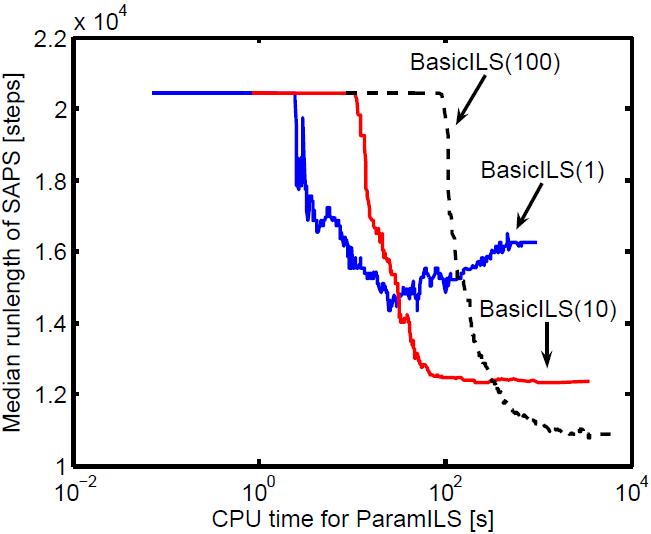
\includegraphics[scale=0.25]{images/basicils.png}}
\only<2>{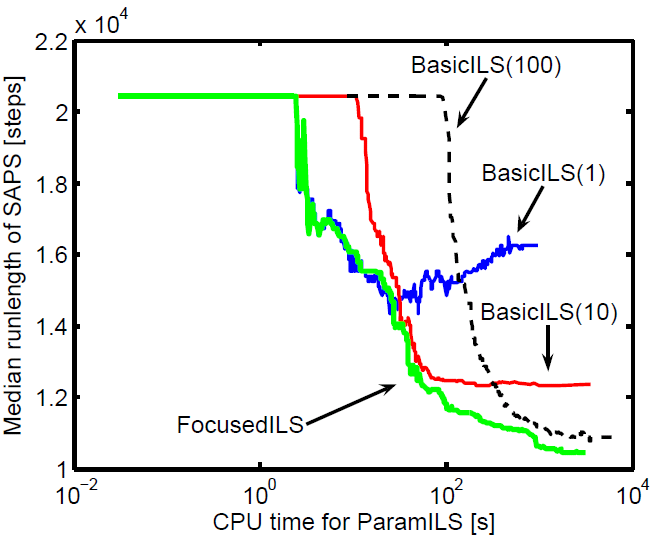
\includegraphics[scale=0.25]{images/focusedils.png}}
\end{center}

\end{frame}
%-----------------------------------------------------------------------



%-----------------------------------------------------------------------
\begin{frame}[c,fragile]{Different Types of Overtuning}

One can overtune to various specifics of the training setup
\begin{itemize}
	\item Overtuning to the specific instances used in the training set 
	\item Overtuning to the specific seeds used in the training set
\pause
	\item Overtuning to the (small) runtime cutoff used during training 
	\item Overtuning to a particular machine type
\pause
	\item Overtuning to the type of instances in the training set
	\begin{itemize}
	  \item These should just be drawn according to the distribution of interest
	  \item But in practice, the distribution might change over time 
	\end{itemize}	 
\end{itemize}	

\pause
\bigskip
Note: We discuss this more in detail in two weeks. 

\end{frame}
%-----------------------------------------------------------------------


\section{Adaptive Capping}

%-----------------------------------------------------------------------
\begin{frame}[c,fragile]{Adaptive capping}

\begin{itemize}
    \item Assumptions
    \begin{itemize} 
      \item optimization of runtime
      \item each configuration run has a time limit (e.g., $300$ sec)
    \end{itemize}
\pause    
    
    \item E.g., $\conf$ needed $1$ sec to solve $\inst_1$
    \begin{itemize}
      \item Do we need to run $\conf'$ for $300$ sec?
      \item Terminate evaluation of $\conf'$ once guaranteed to be worse than $\conf$
    \end{itemize}
\pause
\bigskip    
    \item[$\leadsto$] To compare against $\conf$ based on $N$ runs,\\we can terminate evaluation of $\conf'$ after time $\sum_{i=1}^N m(\conf,\inst_i)$
\end{itemize}

\pause
\begin{theorem}
Adaptive capping does not change the trajectory of \paramils{}, it only makes it faster. 
\end{theorem}

\end{frame}
%-----------------------------------------------------------------------




%-----------------------------------------------------------------------
\begin{frame}[c,fragile]{Toy-Example: Adaptive capping}

runtime cutoff $\kappa = 300$, comparison based on 3 instances (using $\hat{c}_3$)

\begin{center}
\begin{tabular}{l ccc}
 				& $\inst_1$ & $\inst_2$ & $\inst_3$ \\
\hline
$\conf$ 	& 4 		& 2			& 1	\onslide<2->\\
\hline
\multicolumn{3}{l}{\emph{Without adaptive capping}}\\
$\conf'$		& \onslide<3->{3}			& \onslide<4->{300} 		& \onslide<5->{50}\\
				& 			&  & \onslide<6->{$\to$ reject $\conf'$ (\alert{cost: 353})}\onslide<7->\\
\hline
\multicolumn{3}{l}{\onslide<7->{\emph{With adaptive capping}}}\\
%\onslide<5->{$\kappa$}			& \onslide<6->{$4-0=4$}	& \onslide<8->{$6-3=3$} 	& \onslide<10->{$7-5=2$}\\
$\conf'$\onslide<8->			& \onslide<8->{3}		& \onslide<9->{300} 		& \onslide<10->\\
								& 						& \multicolumn{2}{l}{\onslide<10->$\to$ \alert{cut off} after $\kappa=4$ seconds, reject $\conf'$ (\alert{cost: 7})} \\
\hline
\end{tabular}
\end{center}

%\onslide<10->
%$\kappa=4$ seconds: (4+2+1)-3

\end{frame}
%-----------------------------------------------------------------------



\hide{
%-----------------------------------------------------------------------
\begin{frame}[c,fragile]{\paramils{} Results \litw{Hutter et al. 2007,2009}}

\begin{table}
\begin{tabular}{ll cc}
\hline
\hline
Solver & Instances & Default & ParamILS\\
\hline
SAPS & SWGCP & 20.41 & 0.26\\
SPEAR & SWGCP & 9.74 & 6.6\\
SAPS & QCP & 12.97 & 4.29\\
SPEAR & QCP & 2.65 & 1.21\\
CLPEX & REGIONS100 & 1.61 & 0.32\\
\hline
\hline
\end{tabular}

\end{table}

\end{frame}
%-----------------------------------------------------------------------
%-----------------------------------------------------------------------
\begin{frame}[c,fragile]{Results of Adaptive Capping}

TODO

\end{frame}
%-----------------------------------------------------------------------
}




\section{Applications of Algorithm Configuration}



%-------------------------------------------------------------
\begin{frame}[c,fragile]{Configuration of a SAT Solver for Verification}

\begin{block}{SAT (propositional satisfiability problem)}
        \begin{itemize}
                \item Prototypical $\mathcal{NP}$-hard problem
                \item Interesting theoretically and in practical applications
        \end{itemize}
\end{block}
        
\pause

\begin{block}{Formal verification}
        \begin{itemize}
                \item Software verification\\%\refer{Babi\'c \& Hu; CAV '07}
                \item Hardware verification (Bounded model checking) %\refer{Zarpas; SAT '05}
                \item Applications: see Chairs of Profs.\ Becker and Podelski
%                \item[--] Recent progress based on SAT solvers
        \end{itemize}
\end{block}

\pause

\begin{block}{Tree search solver for SAT-based verification}
        \begin{itemize}
                \item SPEAR, developed by Domagoj Babi\'c at UBC
                \item 26 parameters, $8.34 \times 10^{17}$ configurations\\
        \end{itemize}
\end{block}

\end{frame}
%-----------------------------------------------------------------------




%-------------------------------------------------------------
\begin{frame}[c,fragile]{Configuration of a SAT Solver for Verification}
        \onslide<1->
\begin{itemize}
        \item Ran FocusedILS, 2 days $\times$ 10 machines
        \begin{itemize}
                \item[--] On a training set from each benchmark
        \end{itemize}
        \onslide<2->
        
\vspace*{0.0cm}
        \item Compared to manually-engineered default
        \begin{itemize}
                \item[--] 1 week of performance tuning
                \item[--] Competitive with the state of the art
                \item[--] Comparison on unseen test instances
         \end{itemize}

\vspace*{-10mm}
\end{itemize}


\begin{columns}
      \column{0.49\textwidth}
        \begin{center}  
                \onslide<3->
                \includegraphics[width=4cm]{images/lecture11/lci-talk-basic-figures/ibm_default_vs_ibmtuned_w_swapping.pdf}\\
                \alert{$4.5$-fold speedup}\\ on hardware verification
        \end{center}
      \column{0.49\textwidth}
        \begin{center}
                \onslide<4->
                \includegraphics[width=4cm]{images/lecture11/lci-talk-basic-figures/swv_default_vs_swvtuned_w_swapping.pdf}\\        
                \alert{500-fold speedup $\leadsto$ won category QF\_BV in 2007 SMT competition}
        \end{center}
      \column{0.1\textwidth}
\end{columns}                                

%\begin{center}
%\vspace*{-0.5cm}\onslide<4-> Note: lower is better
%\end{center}

\end{frame}
%-----------------------------------------------------------------------



%-------------------------------------------------------------
\begin{frame}[c,fragile]{Configuration of MIP Solvers}

\begin{block}{MIP (mixed integer programming)}
\vspace*{-0.5cm}
\begin{eqnarray}
\nonumber{}min && c^\transpose x\\
\nonumber{}s.t. && Ax \le b\\
\nonumber{}&& x_i \in \mathds{Z} \text{ for } i \in I
\end{eqnarray}
\end{block}

\begin{itemize}
                \item $\mathcal{NP}$-hard optimization problem
                \item Highly relevant in industry
                \begin{itemize}
                       \item IBM ILOG CPLEX licensed by \textgreater\ 1\,300 corporations and 1\,000 universities
\pause 
                       \begin{itemize}
                        \item[-] Transportation and logistics:\\
                        United States Postal Service, UPS, Unites Airlines, SNCF 
                                %(french railway)
%                \fhpause
                                        \smallskip
                        \item[-] Manufacturing:\\
                                Airbus, Dell, Michelin, Porsche, Thyseen Krupp, Toyota
                                %Nissan, 
%                        \fhpause
                        \smallskip
                        \item[-] Supply chain management software vendors:\\
                                Oracle, SAP, Infor, Manhattan Associates, JDA
                        \end{itemize}
                \end{itemize}
\end{itemize}
        \vspace*{0.2cm}



\end{frame}
%-----------------------------------------------------------------------


%\hide{
%From http://www.thefreelibrary.com/ILOG+CPLEX+Optimization+Software+Turns+20.-a0186925142:                
%                Leading organizations worldwide use ILOG optimization tools and, engines to solve the world's most challenging planning and scheduling problems. These customers include APL, BNSF BNSF Burlington Northern Santa Fe Corporation (railroad) , JR East, Logistics, Maersk, Schneider, SNCF SNCF 
% Dell, Hansol Paper, Michelin, Mitsubishi Chemicals, Nippon Steel, Nissan, Porsche, Saint Gobain, Thyssen Krupp, and Toyota in manufacturing. ILOG optimization products are also used by a majority of leading Supply Chain Management software vendors, including Infor, Manhattan Associates, JDA, Oracle, Red Prairie and SAP, as well as in research programs at over 1,000 universities around the world, making the products the "gold standard" for performance and solution quality in the Operations Research community.}
%        }
%}     



%-------------------------------------------------------------
\begin{frame}[c,fragile]{Configuration of MIP Solvers}


\begin{block}{MIP Solvers}
       \begin{itemize}
                \item[--] IBM ILOG CPLEX (76 parameters)
                \item[--] Gurobi (25 parameters)
                \item[--] lpsolve (47 parameters)
        \end{itemize}
\end{block}



\vspace*{-0.1cm}
\pause
\begin{block}{Comparison against algorithm defaults}

\begin{itemize}
                \item[] \emph{``A great deal of algorithmic development effort has been devoted
                      to establishing default ILOG CPLEX parameter settings that 
                      achieve good performance on a wide variety of MIP models.''}\\
                      \refer{\cplex{} 12.1 user manual, page 478}                     
\end{itemize}
\end{block}

\vspace*{-0.1cm}
\pause

\begin{block}{Used six available benchmark distributions, including}
        \begin{itemize}
        		\item Wildlife corridor benchmarks (SUST)
                \item Winner determination in combinatorial auctions (WDP)
                \item Mixed integer knapsack (MIK)
 %               \item Machine-job assignment (MJA)
  %              \item Multi-activity shift scheduling (MASS)
   %             \item Capacitated lot sizing (CLS)
        \end{itemize}
\end{block}

\end{frame}
%-----------------------------------------------------------------------


%-------------------------------------------------------------
\begin{frame}[c,fragile]{Configuration of MIP Solvers: Runtime}

\begin{block}{Min.\ runtime to find optimal solution and prove its optimality}
\begin{itemize}
%        \item Min.\ runtime to find optimal solution and prove its optimality
%        \item To ``optimality'': relative optimality gap of 0.0001 (default)

        \onslide<1->
        \smallskip
        \item For each solver \& dist: ran FocusedILS, 2 days $\times$ 10 machines

        \onslide<2->
        
        \item Mean speedup over default (on test instances)
        \begin{itemize}
                \onslide<3->
                \item[--] IBM ILOG CPLEX 2x to 50x
                \onslide<4->
                \item[--] lpsolve 1x (no speedup) to 150x
                \onslide<5->
                \item[--] Gurobi 1.2x to 2.3x
        \end{itemize}
        
%       \fhpause
\end{itemize}
\end{block}

                \onslide<1->
\vspace*{-4mm}

  \begin{columns}
      \column{.5\textwidth}
        \begin{center}                  
                \only<3-5>{
\includegraphics[width=3.0cm]{images/lecture11/mip-results/runtime-opt/cplex_scatter-plot-CL-2days-300s-PAR1086400.pdf}\\
                                \footnotesize{\cplex{} on SUST instances (50x)}}
%                \only<6>{
%\includegraphics[height=4cm,width=4.5cm]{figures/mip-results/runtime-opt/gurobi_scatter-plot-MIK-2days-PAR10-300s86400.pdf}\\
%                                \footnotesize{\gurobi{} on MIK instances (1.2x)}
%                }               
        \end{center}
    \column{.5\textwidth}
        \begin{center}                  
                \only<4>{
\includegraphics[width=3.0cm]{images/lecture11/mip-results/runtime-opt/lpsolve_scatter-plot-CATS200-300s-2days-PAR1086400.pdf}\\
                                \footnotesize{\lpsolve{} on WDP instances (150x)}}
%                 \only<5>{
% \includegraphics[width=3.0cm]{images/lecture11/mip-results/runtime-opt/gurobi_scatter-plot-CL-2days-PAR10-300s86400.pdf}\\
%                                 \footnotesize{\gurobi{} on SUST instances (2.3x)}               
%                 }               
        \end{center}
  \end{columns}


\end{frame}
%-----------------------------------------------------------------------


%-------------------------------------------------------------
\begin{frame}[c,fragile]{Configuration of MIP Solvers: Optimality Gap}

\begin{block}{Minimize optimality gap reachable in 10 seconds}
\begin{itemize}
        \item Ran FocusedILS for 5 hours on 10 machines
        
%        \fhpause
%        \smallskip

        \item Reduction factors of average optimality gap (on test inst.)
        \begin{itemize}
                \item[--] IBM ILOG CPLEX 1.3x to 8.6x
                \item[--] Gurobi 1.1x to 2.2x
                \item[--] lpsolve 1x (no reduction) to 46x
        \end{itemize}
\end{itemize}
\end{block}
        
\pause        
\vspace*{-0.6cm} 
    \begin{columns}
      \column{.5\textwidth}
                                \begin{center}  \includegraphics[height=4cm,width=4.5cm]{images/lecture11/mip-results/mipgap-opt/cplex_scatter-plot-MIK-qualtie-5h-10s10000.pdf}\\
                                \footnotesize{\cplex{} on MIK instances (8.6x)}
                                \end{center}
%                               \fhpause
      \column{.5\textwidth}
                                \begin{center}  \includegraphics[height=4cm,width=4.5cm]{images/lecture11/mip-results/mipgap-opt/lpsolve_scatter-plot-MIK-qualtie-5h-10s10000.pdf}\\
%                               \begin{center}  \includegraphics[height=2.8cm,width=3.4cm]{figures/lci-talk-basic-figures/swv_default_vs_swvtuned_w_swapping.pdf}\\
                                \footnotesize{\lpsolve{} on MIK instances (46x)}% \refer{Babi\'c \& Hu; CAV '07}}
                                \end{center}
    \end{columns}
\end{frame}
%-----------------------------------------------------------------------


%-------------------------------------------------------------
\begin{frame}[c,fragile]{Comparison to CPLEX Tuning Tool}

\begin{itemize}

        \item IBM ILOG CPLEX tuning tool
        \begin{itemize}
                \item[--] Introduced in version 11 (late 2007, after \paramils{})
                \item[--] Evaluates predefined good configurations, returns best one
                \item[--] Required runtime varies (from $< 1h$ to weeks)
        \end{itemize}
        \onslide<3->
        \item \paramils{}: anytime algorithm
        \begin{itemize}
                \item[--] At each time step, keeps track of its incumbent
        \end{itemize}
        \onslide<1->
\end{itemize}

\vspace*{-0.5cm}

    \begin{columns}
      \column{.5\textwidth}
                                \begin{center}          
%                                \only<1>{\vspace*{4cm}}                               %\only<3>{\includegraphics[height=4cm,width=4.5cm]{figures/mip-results/vs_cplex_tuning_tool/cplex_overtime-MIK-36307-10000-PAR1086400fig-onlydef.pdf}\\}
\only<2-3>{\includegraphics[width=4.0cm]{images/lecture11/mip-results/vs_cplex_tuning_tool/cplex_overtime-MIK-36307-10000-PAR1086400.pdf}\\\footnotesize{\cplex{} on MIK instances}}
                                \end{center}
                                \pause
      \column{.5\textwidth}
                                \begin{center}          
                                \onslide<3>
\includegraphics[width=4.0cm]{images/lecture11/mip-results/vs_cplex_tuning_tool/cplex_overtime-TUNE12-CL-172800-10000-PAR1086400.pdf}\\
%                               \begin{center}  \includegraphics[height=2.8cm,width=3.4cm]{figures/lci-talk-basic-figures/swv_default_vs_swvtuned_w_swapping.pdf}\\
                                \footnotesize{\cplex{} on SUST instances}% \refer{Babi\'c \& Hu; CAV '07}}
                                \end{center}
    \end{columns}

\begin{center}
\onslide<2->Note: lower is better
\end{center}
\end{frame}
%-----------------------------------------------------------------------



%----------------------------------------------------------------------
\begin{frame}[c]{Summary by Learning Goals}

Now, you should be able to \ldots

\begin{itemize}
  \item \alert{formally} define the algorithm configuration problem and discuss its
  complexity
  \item explain the \alert{overtuning} phenomenon and how to avoid it
%\pause
\medskip
  \item motivate \& describe the algorithm configuration framework \alert{\paramils{}}
  \item motivate \alert{FocusedILS} and prove its \alert{convergence} property
  \item describe the concept of \alert{adaptive capping}  
%\pause
\medskip
  \item describe \alert{application examples} for algorithm configuration
%  \item sketch the ideas of the configurators \gga{} and \irace{}
\end{itemize}
\end{frame}
%----------------------------------------------------------------------



%-----------------------------------------------------------------------
\begin{frame}[c,fragile]{Further Reading (these are hyperlinks)}

\begin{itemize}
	\item \href{http://aad.informatik.uni-freiburg.de/papers/09-JAIR-ParamILS.pdf}{\alert{ParamILS journal paper}: introduction to algorithm configuration, ParamILS, adaptive capping; long, but easy to read.}
	\item \href{http://aad.informatik.uni-freiburg.de/papers/07-AAAI_ParamILS.pdf}{\alert{ParamILS conference paper}:\\good reference for overtuning, but otherwise very terse presentation} 

	\item Applications:
	\begin{itemize}
	  \item \href{http://aad.informatik.uni-freiburg.de/papers/07-fmcad-BoostingVerification.pdf}{Formal verification (Spear)}
	  \item \href{http://aad.informatik.uni-freiburg.de/papers/10-CPAIOR-MIP-Config.pdf}{Mixed integer programming (IBM ILOG CPLEX)}
	  \item \href{icaps11.icaps-conference.org/proceedings/pal/vallati-et-al.pdf}{AI planning (LPG)}
	  \item \href{https://www.cs.ubc.ca/cgi-bin/tr/2009/TR-2009-15.pdf}{Time tabling (UBCTT)}
	  \item \href{http://www.cs.ubc.ca/labs/beta/Projects/autoweka/papers/autoweka.pdf}{Supervised learning (Auto-WEKA)}
	\end{itemize}
\end{itemize}

\end{frame}
%-----------------------------------------------------------------------
